\section{Modelos de Regresi??n}

Finalmente, vemos los modelos propuestos. Primero sin la libertad mundial como independiente, y luego con est??. Los resultados se muestran en la Tabla \ref{regresiones} de la p??gina \pageref{regresiones}.




% Table created by stargazer v.5.2.2 by Marek Hlavac, Harvard University. E-mail: hlavac at fas.harvard.edu
% Date and time: Fri, Jun 29, 2018 - 16:15:49
\begin{table}[!htbp] \centering 
  \caption{Modelos de Regresi??n} 
  \label{regresiones} 
\begin{tabular}{@{\extracolsep{5pt}}lcc} 
\\[-1.8ex]\hline 
\hline \\[-1.8ex] 
 & \multicolumn{2}{c}{\textit{Dependent variable:}} \\ 
\cline{2-3} 
\\[-1.8ex] & \multicolumn{2}{c}{Democracy} \\ 
\\[-1.8ex] & (1) & (2)\\ 
\hline \\[-1.8ex] 
 WorldFreedom &  & 0.704$^{***}$ \\ 
  &  & (0.046) \\ 
  & & \\ 
 EconomicFreedom & 0.377$^{***}$ & 0.291$^{***}$ \\ 
  & (0.077) & (0.053) \\ 
  & & \\ 
 PressFreedom & 0.833$^{***}$ & 0.012 \\ 
  & (0.065) & (0.070) \\ 
  & & \\ 
 Constant & $-$0.642$^{***}$ & $-$0.354$^{**}$ \\ 
  & (0.199) & (0.138) \\ 
  & & \\ 
\hline \\[-1.8ex] 
Observations & 206 & 206 \\ 
R$^{2}$ & 0.637 & 0.830 \\ 
Adjusted R$^{2}$ & 0.634 & 0.828 \\ 
Residual Std. Error & 0.880 (df = 203) & 0.603 (df = 202) \\ 
F Statistic & 178.197$^{***}$ (df = 2; 203) & 329.420$^{***}$ (df = 3; 202) \\ 
\hline 
\hline \\[-1.8ex] 
\textit{Note:}  & \multicolumn{2}{r}{$^{*}$p$<$0.1; $^{**}$p$<$0.05; $^{***}$p$<$0.01} \\ 
\end{tabular} 
\end{table} 
Como se vi?? en la Tabla \ref{regresiones}, cuando est?? presente el \emph{indice de libertad mundial}, el \emph{??ndice de libertad de prensa} pierde significancia.

\clearpage

\section{Exploraci??n Espacial}

Como acabamos de ver en la Tabla \ref{regresiones} en la p??gina \pageref{regresiones}, si quisieras sintetizar la multidimensionalidad de nuestros indicadores, podr??amos usar tres de las cuatro variables que tenemos (un par de las originales tiene demasiada correlaci??n). 

As??, propongo que calculemos conglomerados de pa??ses usando toda la informaci??n de tres de los indicadores. Como nuestras variables son ordinales utilizaremos un proceso de conglomeraci??n donde las distancia ser??n calculadas usando la medida {\bf gower} propuestas en \cite{gower_general_1971}, y para los enlazamientos usaremos la t??cnica de {\bf medoides} seg??n \cite{reynolds_clustering_2006}. Los tres conglomerados se muestran en la Figura \ref{clustmap}.






\begin{figure}[h]
\centering
\begin{adjustbox}{width=11cm,height=8cm,clip,trim=1cm 2.5cm 0cm 2.5cm}
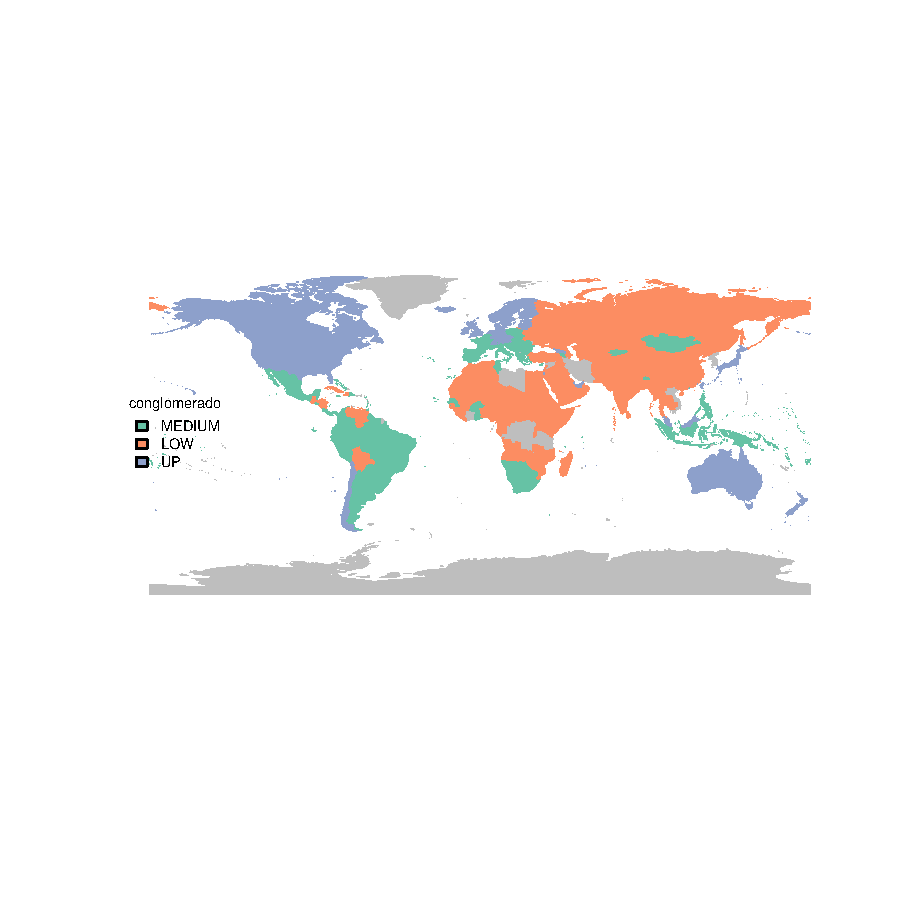
\includegraphics{paperVersion_7_regresion-plotMap1}
\end{adjustbox}
\caption{Paises conglomerados segun sus indicadores sociopol??ticos}\label{clustmap}
\end{figure}



\endinput
